\documentclass[10pt,a4paper]{article}
\usepackage[margin=1in]{geometry}
\usepackage{tikz}
\usepackage{fontspec}
\usepackage{xcolor}

\definecolor{accent}{RGB}{60, 60, 60}
\definecolor{lightgray}{RGB}{200, 200, 200}

\begin{document}
\thispagestyle{empty}

% Background decorative elements

\begin{tikzpicture}[overlay, remember picture]
    % Left vertical bar
    \fill[black] 
        ([xshift=1.5cm, yshift=-2cm]current page.north west) 
        rectangle 
        ([xshift=1.7cm, yshift=2cm]current page.south west);
    
    % Bottom accent line
    \draw[line width=2pt, color=black] 
        ([yshift=2cm]current page.south west) -- 
        ([yshift=2cm]current page.south east);
    
    % Top thin line
    \draw[line width=1pt, color=lightgray] 
        ([yshift=-2cm]current page.north west) -- 
        ([xshift=-2cm, yshift=-2cm]current page.north east);
    
    % Corner squares
    \fill[black] ([xshift=2cm, yshift=-2.3cm]current page.north west) rectangle ++(0.4, -0.4);
    \fill[black] ([xshift=2cm, yshift=2.3cm]current page.south west) rectangle ++(0.4, 0.4);
    \fill[black] ([xshift=-2.4cm, yshift=-2.3cm]current page.north east) rectangle ++(-0.4, -0.4);
    \fill[black] ([xshift=-2.4cm, yshift=2.3cm]current page.south east) rectangle ++(-0.4, 0.4);
\end{tikzpicture}

\vspace*{1.5cm}

% Course Title
\begin{center}
    {\fontsize{32}{38}\selectfont \textbf{ECONOMICS}}\\[0.5cm]
    {\fontsize{16}{20}\selectfont \textcolor{accent}{COMPREHENSIVE COURSE NOTES}}\\[1.5cm]
    
    % Decorative line
    
\begin{tikzpicture}
        \draw[line width=1pt] (0,0) -- (3,0);
        \filldraw (1.5,0) circle (2pt);
        \draw[line width=1pt] (4.5,0) -- (7.5,0);
        \filldraw (6,0) circle (2pt);
    \end{tikzpicture}
    \vspace{1.5cm}
    
    % Course Description
    {\fontsize{12}{16}\selectfont This document contains a complete set of economics notes}\\[0.3cm]
    {\fontsize{12}{16}\selectfont covering all major topics in microeconomics and macroeconomics.}\\[0.3cm]
    {\fontsize{12}{16}\selectfont Each topic is presented in a structured two-column format with:}\\[1.5cm]
    
    % Features Boxes
    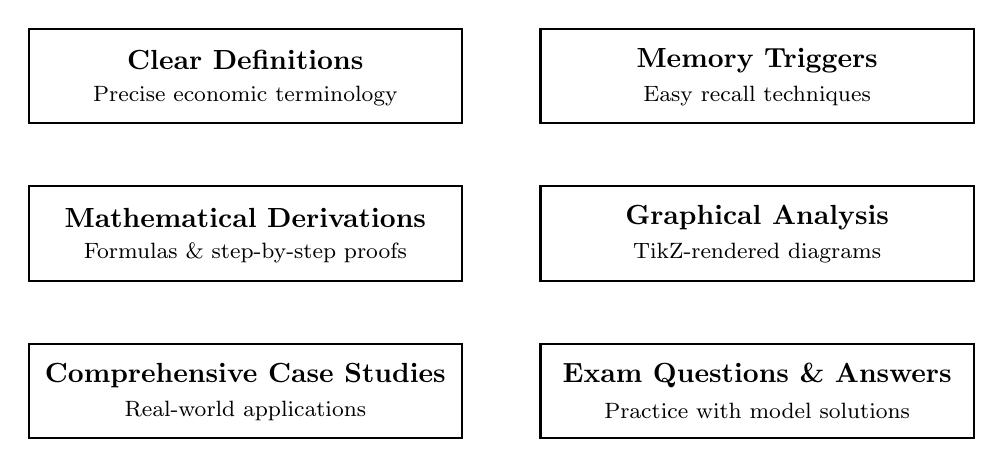
\begin{tikzpicture}
        % Row 1
        \draw[thick] (0,0) rectangle (5.5,1.2);
        \node[font=\normalsize\bfseries] at (2.75,0.8) {Clear Definitions};
        \node[font=\footnotesize] at (2.75,0.35) {Precise economic terminology};
        
        \draw[thick] (6.5,0) rectangle (12,1.2);
        \node[font=\normalsize\bfseries] at (9.25,0.8) {Memory Triggers};
        \node[font=\footnotesize] at (9.25,0.35) {Easy recall techniques};
        
        % Row 2
        \draw[thick] (0,-2) rectangle (5.5,-0.8);
        \node[font=\normalsize\bfseries] at (2.75,-1.2) {Mathematical Derivations};
        \node[font=\footnotesize] at (2.75,-1.65) {Formulas \& step-by-step proofs};
        
        \draw[thick] (6.5,-2) rectangle (12,-0.8);
        \node[font=\normalsize\bfseries] at (9.25,-1.2) {Graphical Analysis};
        \node[font=\footnotesize] at (9.25,-1.65) {TikZ-rendered diagrams};
        
        % Row 3
        \draw[thick] (0,-4) rectangle (5.5,-2.8);
        \node[font=\normalsize\bfseries] at (2.75,-3.2) {Comprehensive Case Studies};
        \node[font=\footnotesize] at (2.75,-3.65) {Real-world applications};
        
        \draw[thick] (6.5,-4) rectangle (12,-2.8);
        \node[font=\normalsize\bfseries] at (9.25,-3.2) {Exam Questions \& Answers};
        \node[font=\footnotesize] at (9.25,-3.65) {Practice with model solutions};
    \end{tikzpicture}
    
    \vspace{2cm}
    
    % Topics Overview
    {\fontsize{13}{17}\selectfont \textbf{Topics Covered}}\\[1cm]
    
    \begin{tabular}{p{4.5cm} p{4.5cm} p{4.5cm}}
        \textbullet\ Basic Economic Concepts & \textbullet\ Demand \& Supply & \textbullet\ Elasticity \\
        \textbullet\ Consumer Behavior & \textbullet\ Indifference Curves & \textbullet\ Production \& Cost \\
        \textbullet\ Firm Decisions & \textbullet\ Market Structures & \textbullet\ Macroeconomics \\
        \textbullet\ GDP \& National Income & \textbullet\ Inflation \& Unemployment & \textbullet\ Fiscal \& Monetary Policy \\
    \end{tabular}
    
    \vspace{2cm}
    
    % Decorative line
    
\begin{tikzpicture}
        \draw[line width=1pt] (0,0) -- (3,0);
        \filldraw (1.5,0) circle (2pt);
        \draw[line width=1pt] (4.5,0) -- (7.5,0);
        \filldraw (6,0) circle (2pt);
    \end{tikzpicture}
    \vspace{1cm}
    
    % Bottom note
    {\fontsize{10}{13}\selectfont \textcolor{accent}{\textit{Designed for efficient learning \& quick revision}}}\\[0.3cm]
    {\fontsize{10}{13}\selectfont \textcolor{accent}{\textit{Academic Year 2024--2025}}}
    
\end{center}

% Bottom bar
\begin{tikzpicture}[overlay, remember picture]
    \fill[black] 
        ([xshift=1.5cm, yshift=0.5cm]current page.south west) 
        rectangle 
        ([xshift=-1.5cm, yshift=0.8cm]current page.south east);
    \node[text=white, font=\footnotesize] 
        at ([yshift=0.65cm]current page.south) 
        {Typeset in \LaTeX\ | Two-Column Layout | Black \& White Format};
\end{tikzpicture}

\vspace*{0.8cm}

\end{document}